% =====================================================================
%  EV-PRAC-01 · Ingeniería de Requerimientos (ISR-401) · UTEQ
%  Transcripción fiel de la prueba escrita a mano (3 hojas)
%  Regla R2: el texto se copia tal cual, con su ortografía original.
% =====================================================================
\documentclass[11pt,a4paper]{article}

\usepackage[utf8]{inputenc}
\usepackage[T1]{fontenc}
\usepackage[spanish]{babel}
\usepackage[margin=2.5cm]{geometry}
\usepackage{array}
\usepackage{tabularx}
\usepackage{graphicx}
\usepackage{xcolor}
\usepackage{float}
\usepackage{hyperref}

% Los enunciados se escribieron en rojo en las hojas
\newcommand{\enun}[1]{\textcolor{red}{#1}}
\newcolumntype{C}{>{\centering\arraybackslash}X}
\renewcommand{\arraystretch}{1.25}
\setlength{\parindent}{0pt}
\setlength{\parskip}{6pt}

\begin{document}

% Declaración obligatoria (regla R5)
\noindent\fbox{\parbox{\dimexpr\linewidth-2\fboxsep-2\fboxrule}{%
Esta es la transcripción fiel de la prueba escrita a mano el 18/11/2026;
las fotografías de las hojas están en el anexo.}}

\bigskip

% =========================== HOJA 1 ==================================

\begin{center}
\enun{\large Examen de Ingenieria de requerimientos}
\end{center}

\enun{Nombre: Erick Monserrate Ochoa}\\
\enun{Fecha: 18/11/2026}

\enun{a) Explique con sus palabras qué es un requisito según ISO/IEC/IEEE 29148 y, con esa
explicación, decida si E7 y E12 son requisitos del producto FRÍOVAC.}

El requisito es una necesidad o condición que debe cumplir un sistema de forma clara y
verificable.

E7: No es requisito describe el registro manual activo.

E12: No es requisito porque no es una necesidad o condición que el software necesite.

\enun{b) Explique qué describe la especificación de requisitos de los interesados (StRS), la
especificación de requisitos del sistema (SyRS) y la especificación de requisitos del
software (SRS)}

\begin{center}
\begin{tabularx}{\linewidth}{l l X}
E1  & StRS & Porque es un requisito que lo dan los interesados en el sistema \\
E10 & SyRS & Porque engloba todo tanto software como a los agentes externos \\
E5  & SRS  & Porque es algo que el software hará \\
\end{tabularx}
\end{center}

% =========================== HOJA 2 ==================================

\enun{c) Para cada hecho H1 a H5 indique a qué actividad del proceso de IR corresponde
(elicitación, análisis y negociación, especificación, validación o gestión) y si en el
marco de Pohl es una actividad central o transversal.}

\begin{center}
\begin{tabularx}{\linewidth}{|l|C|C|}
\hline
H1 & Elicitacion            & Central \\ \hline
H2 & Analisis y negociacion & Central \\ \hline
H3 & Especificacion         & Central \\ \hline
H4 & Validación             & Central \\ \hline
H5 & Gestión                & Transversal \\ \hline
\end{tabularx}
\end{center}

\enun{T2. Clasificación y auditoría}

\enun{a) Clasificación. Dibuje una tabla con las columnas ID, Tipo, Documento y
Justificación, y complétela para E1 a E12. Tipo: funcional; no funcional (diga la
característica de ISO/IEC 25010:2023); restricción; requisito de dominio}

\begin{center}
\begin{tabularx}{\linewidth}{|c|C|C|C|}
\hline
ID  & Tipo            & Documento & Justificacion \\ \hline
E1  & Funcional       & StRS      & Necesidad del software para controlar temp \\ \hline
E2  & Req. Dominio    & SyRS      & Necesidad del sistema para medir y controlar \\ \hline
E3  & Restricciones   & SyRS      & Impone un sensor \\ \hline
E4  & Restriccion     & Ninguno   & - \\ \hline
E5  & Funcional       & SRS       & Funcion del Software \\ \hline
E6  & No Funcional    & SyRS      & Son Eficientes \\ \hline
E7  & No es requisito & Ninguno   & No es \\ \hline
E8  & No Funcional    & SRS       & Eficiencia obra de calidad \\ \hline
% ----------------------- aquí empieza la HOJA 3 ----------------------
E9  & Restriccion     & SRS       & \\ \hline
E10 & No Funcional    & SRS       & \\ \hline
E11 & No Funcional    & SRS       & \\ \hline
E12 & Proceso         & Ninguno   & \\ \hline
\end{tabularx}
\end{center}

% =========================== HOJA 3 ==================================

\enun{b) Auditoría. Dibuje una tabla con las columnas ID, Término o construcción
problemática}

\begin{center}
\begin{tabularx}{\linewidth}{|c|C|C|C|}
\hline
ID & Termino o Construcción problematica & Caracteristica & Smart Just \\ \hline
B1 & Ambiguo             & No es medible              & \\ \hline
B2 & Sin destinatorio    & Especifico y medible       & \\ \hline
B3 & Factible y correcto & Alcanzable y realizable    & \\ \hline
B4 & Ninguno Infraccion  &                            & \\ \hline
B5 & No ambiguo          & Especifico y medible       & \\ \hline
B6 & Ninguno Infraccion  & Cumple propiedades basicas & \\ \hline
\end{tabularx}
\end{center}

\enun{T3. Redacción de requisitos bien formados}

\begin{center}
\begin{tabularx}{\linewidth}{|c|C|C|c|C|c|}
\hline
ID  & Enunciado & Tipo & Documento & Fuente & Verificas \\ \hline
B1a & Cuando existan 50 usuarios conectados & No funcional & SRS & B1, E8 & Prueba \\ \hline
B1b & Cuando un responsable utilice la aplicación por primera vez & No funcional & SRS & B1, E11 & Demostración \\ \hline
B2  & Cuando el sensor & Funcional & SRS & B2, E1, E2, B6 & Prueba \\ \hline
B3  & Durante un corte & Funcional & SyRS & B3, E3, E6 & Prueba \\ \hline
B5  & Cuando la coordinadora & Funcional & SRS & B5 & Demostracion \\ \hline
\end{tabularx}
\end{center}

% =====================================================================
% ANEXO — fotografías de las hojas
% =====================================================================
\clearpage
\section*{Anexo: fotografías de las hojas}

\begin{figure}[H]
  \centering
  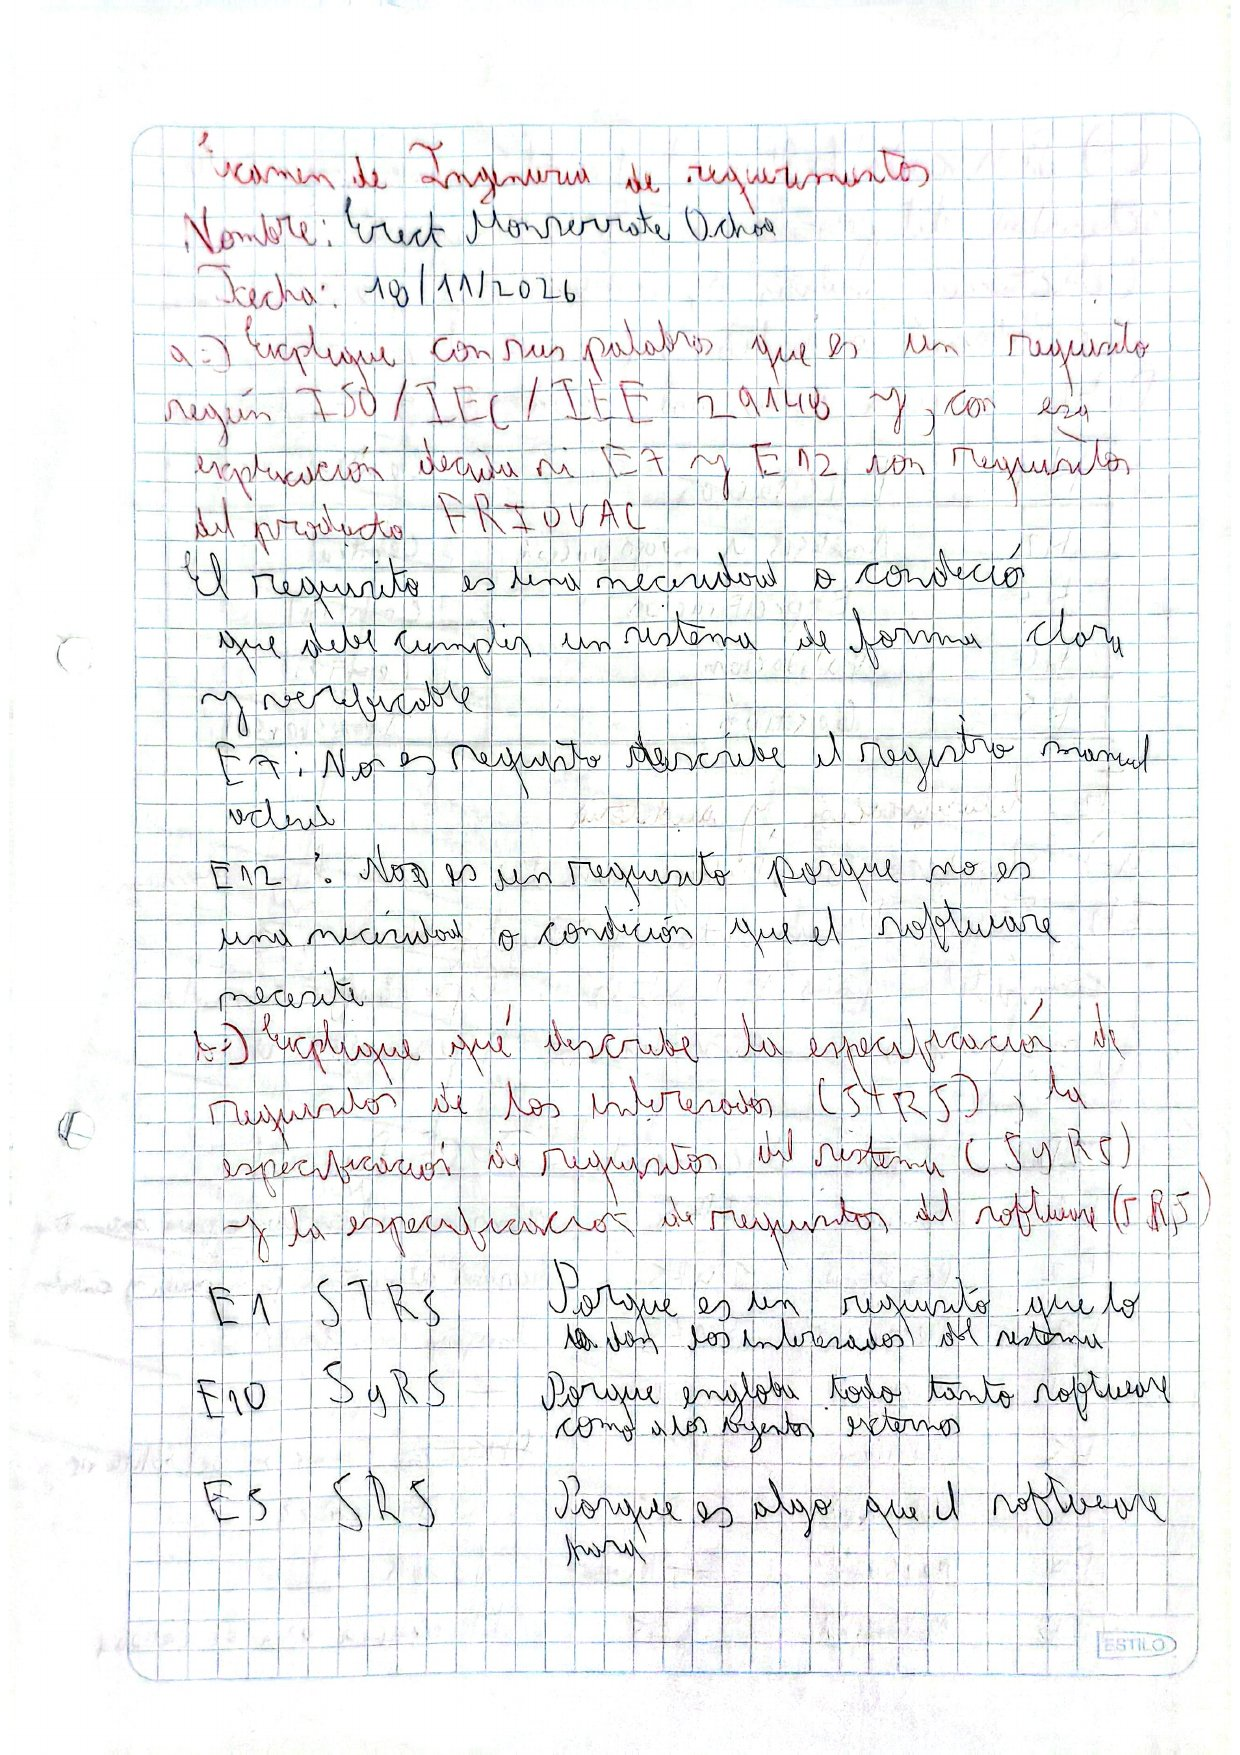
\includegraphics[width=\linewidth,height=0.85\textheight,keepaspectratio]{evidencias/hoja-01.jpg}
  \caption*{Hoja 1 de 3}
\end{figure}
\clearpage
\begin{figure}[H]
  \centering
  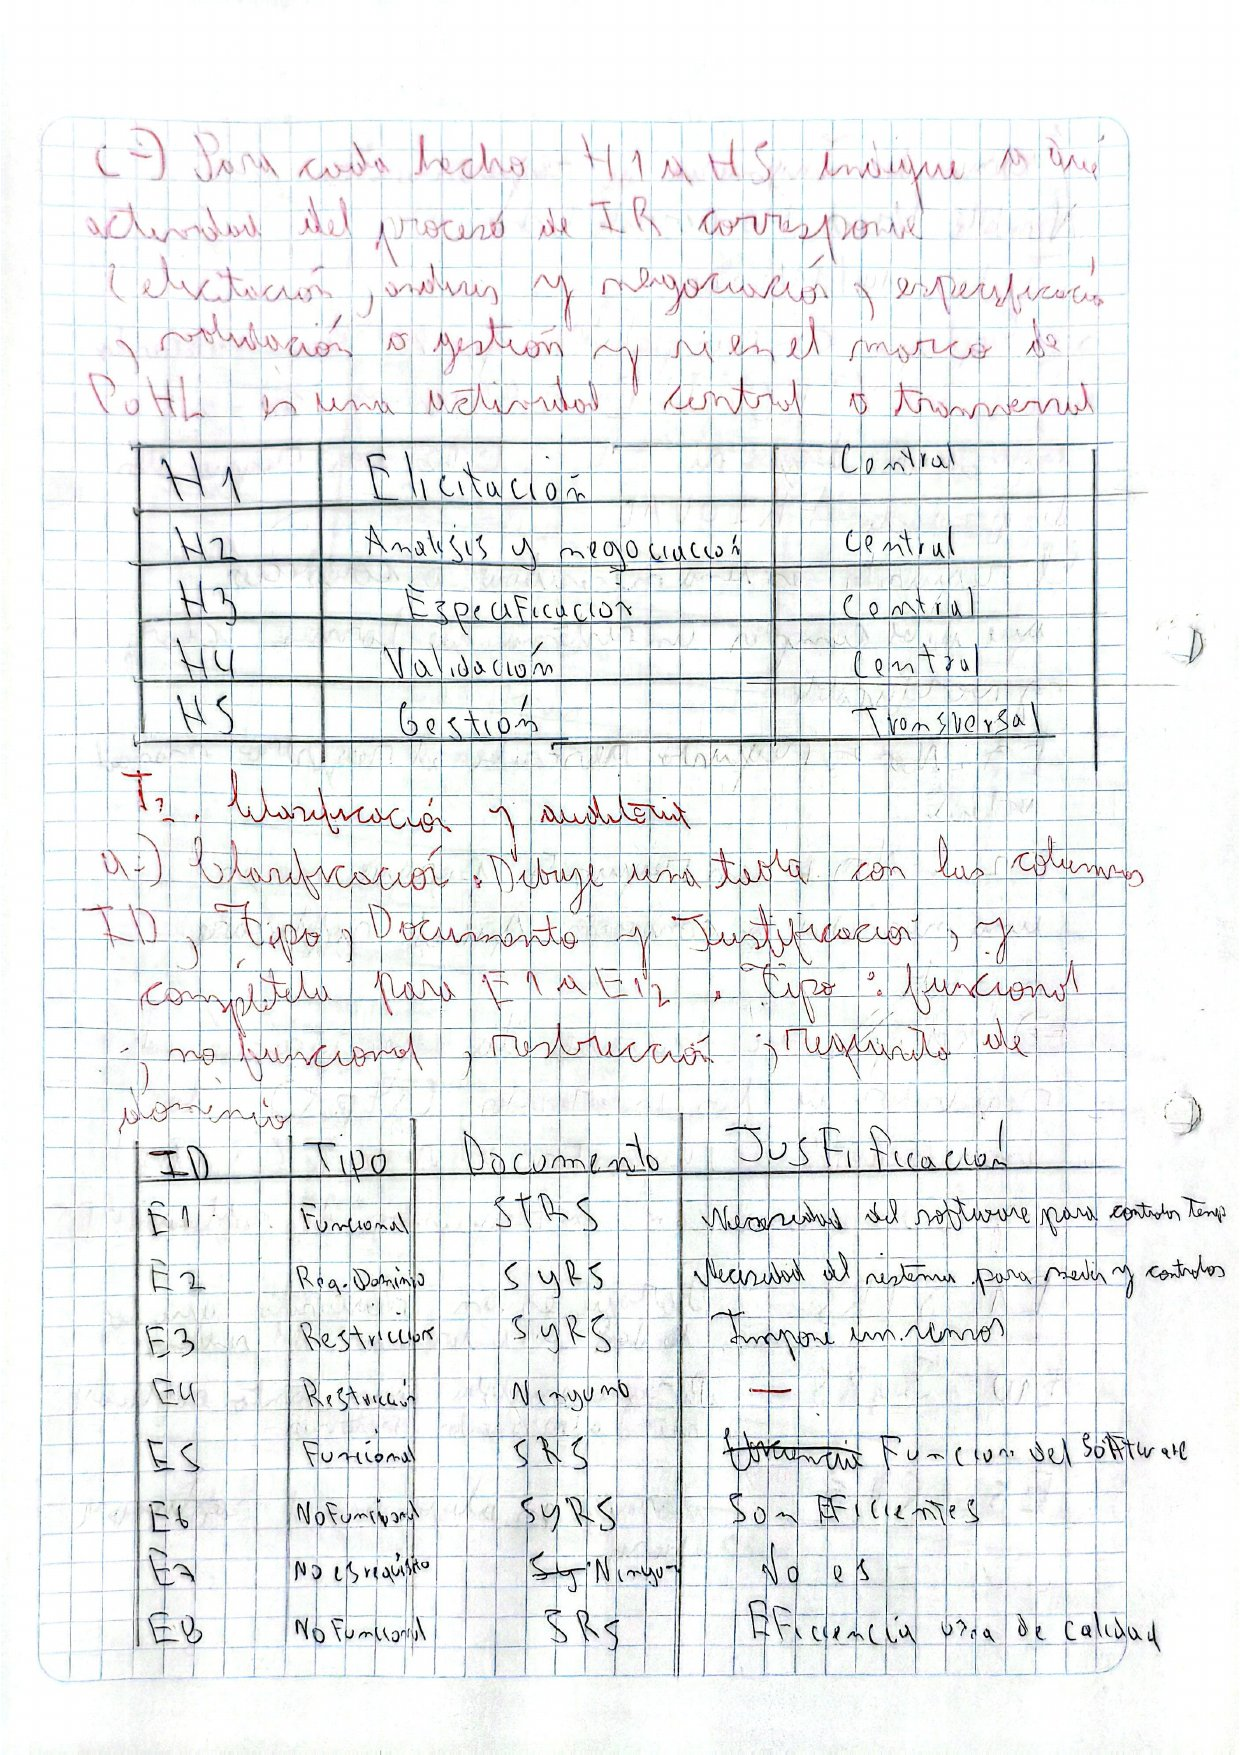
\includegraphics[width=\linewidth,height=0.85\textheight,keepaspectratio]{evidencias/hoja-02.jpg}
  \caption*{Hoja 2 de 3}
\end{figure}
\clearpage
\begin{figure}[H]
  \centering
  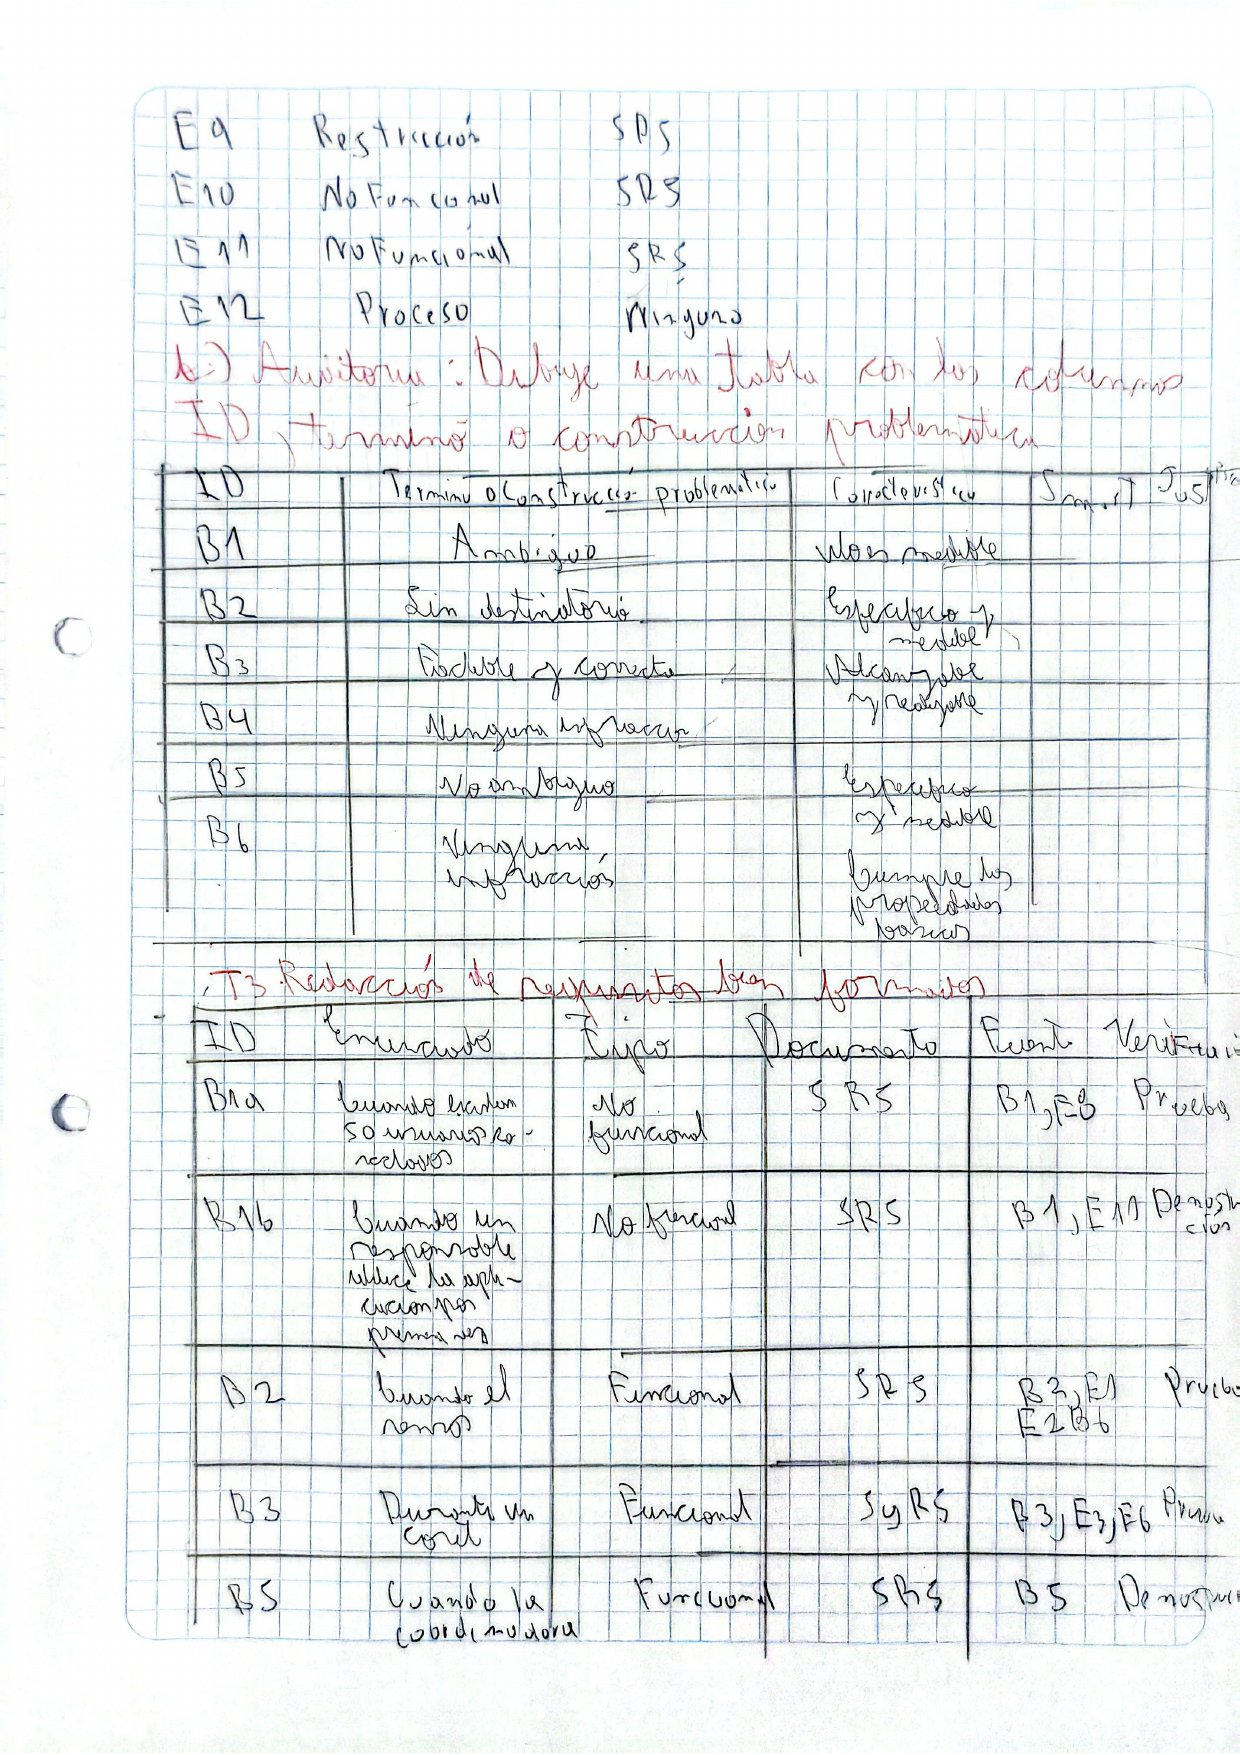
\includegraphics[width=\linewidth,height=0.85\textheight,keepaspectratio]{evidencias/hoja-03.jpg}
  \caption*{Hoja 3 de 3}
\end{figure}

\end{document}
